\section{Methodik}


\subsection{Allgemeiner Aufbau}


\subsubsection{Vorgaben von Faber}

\begin{itemize}
	\item Was will man visualiseren?
	\begin{itemize}
		\item Magnetischerfluss von Flüssigem metall in kokune
		\item Soll dabei helfen die einlaufgeschwindigkeit zu regulieren
	\end{itemize}
	
	\item Geschlossenes netzwerk
	\begin{itemize}
		\item Kein Internet zugriff
	\end{itemize}
	
	\item Möglichkeit der filterung der visuellen Ergebnisse
	\item Soll auf Handy ohne Einstellungen laufen\\
		("Einfach auf website gehen und LETS GOOOOOO")
\end{itemize}


\subsubsection{Probleme / Abweichungen von den Vorgaben}

\begin{itemize}
	\item HTTPS erforderlich für kamera
	\begin{itemize}
		\item Lokaler Host Server braucht SSL zertifikat - Manuelle trustung des Zertifikats am handy unumgänglich
	\end{itemize}
	
	\item HTTPS oder unsecured source Einstellung für backend kommunikation erforderlich
	\item=> Für Beispielzwecke beides HTTPS via Internet
\end{itemize}


\subsubsection{Komponenten}

\begin{itemize}
	\item Backend vs. Frontend
	\begin{itemize}
		\item Frontend: AR visualisierung (allgemein)
		\item Backend: Implementierungs spezifizierung
		\item ziel: Frontend kann mit verschiedenen Backends genutzt werden
	\end{itemize}
\end{itemize}


\subsection{Visualisierung/Frontend}

\begin{figure}
	\centering
	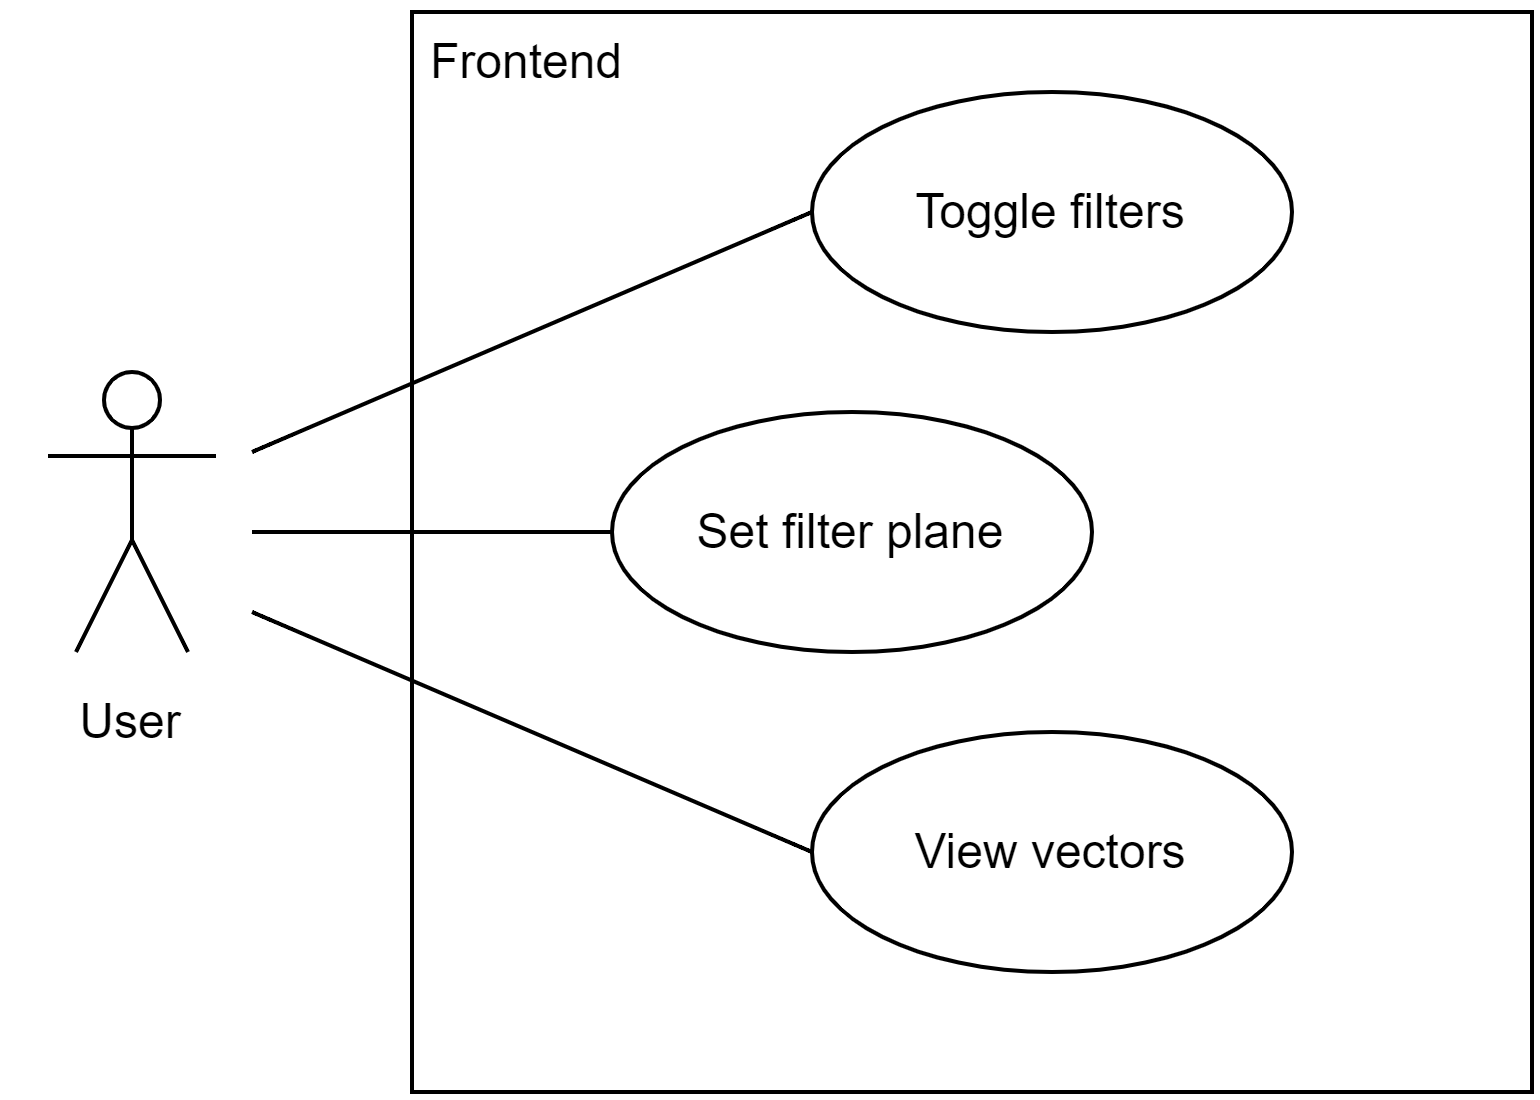
\includegraphics[width=.75\linewidth]{images/frontend/UseCases}
	\caption{Frontend use cases.}
	\label{fig:frontendUseCase}
\end{figure}

\begin{itemize}
	\item Abbildung \ref{fig:frontendUseCase} zeigt
		die Möglichkeiten des Frontends.
	\begin{itemize}
		\item Filtern
		\item Anzeigen
	\end{itemize}
	
	\item Three.js + AR.js
	\begin{itemize}
		\item OpenGL
	\end{itemize}

	\item Auswahl von Filter-Parametern
	\item Object-Tree:
	\begin{itemize}
		\item Marker-Origin (wird von AR.js verschoben -> auf Marker in Quelle)
		\begin{itemize}
			\item Welt-Origin (korrigiert Marker verschiebung+rotation+skalierung von welt-origin)
			\begin{itemize}				
				\item Kokille Modell
				\item Pfeile (10000 * ArrowHelper)
				\item Filter-Box
			\end{itemize}
		\end{itemize}
	\end{itemize}
\end{itemize}



\subsection{Daten bereitstellung/Backend}

\begin{enumerate}
	\item REST (REST conforme endpunkte)
	\item JSON (quote his paper)
	\item Aufbau
	\begin{itemize}
		\item Architektur
		\begin{itemize}
			\item Endpunkte (evtl als diagram (Usecase))
			\begin{itemize}
				\item GET /api/data
				\begin{itemize}
					\item Gibt Vector Daten im JSON format zurück
				\end{itemize}
				
				\item GET /api/data/v2
				\begin{itemize}
					\item Gibt Vector Daten im JSON format zurück und unterstützt filterung
				\end{itemize}
				
				\item GET /api/data/meta
				\begin{itemize}
					\item Gibt Informationen über zur verfügung gestellte daten zurück
					\item (anzahl vektoren im Datensatz, min \& max werte für axen)
				\end{itemize}
			\end{itemize}
			
			\item Hosten der Static files
			\begin{itemize}
				\item /hiro.patt
				\item /kokilleTransformation.JSON
				\item /positioning.JSON
				\item /camera\_para.dat
				\begin{itemize}
					\item allgemeine camera parameter (von AR js mit ausgesendet)
					\item idealterweise jede camera eigene parameter (utopie)
				\end{itemize}
				
				\item /model
				\begin{itemize}
					\item /kokille.mtl
					\item /kokille.obj
				\end{itemize}
			\end{itemize}
		\end{itemize}
			
		\item CORS
		\begin{itemize}
			\item Nötig damit api von anderen websiten aufgerufen werden kann
			\item Prinzip:
			\begin{itemize}
				\item Client schickt Origin Header mit
				\item Wenn Origin zu der liste der zugelassenen Hosts ist wird bei der antwort der Allow-Origin Header gesetzt
			\end{itemize}
		\end{itemize}
	\end{itemize}
\end{enumerate}



